\chapter{Algarismos Significativos}
\label{algSig}
\vspace{-0.5cm}
Imagine que você pergunta a hora a uma pessoa com um relógio de pulso analógico, como o mostrado na Figura~\ref{fig:relogio}. Essa pessoa dá uma olhada no relógio,  e responde: são 10 horas e 42 minutos. Voc\^e entende que o ponteiro dos minutos certamente estava entre o 8 e o 9, ou seja, corresponde a um valor entre 40 e 45 minutos, mais pr\'oximo de 40 do que de 45. Dizemos que esse algarismo que foi estimado, o 2,  \'e um {\bf algarismo duvidoso}. Os outros algarismos são {\bf algarismos certos}: o ponteiro das horas estava entre 10 e 11, com certeza. O conjunto de algarismos certos e duvidosos são os {\bf algarismos significativos da medida}. Quanto maior for o número de algarismos significativos em uma medida, mais informação ela traz. 

\vspace{-0.5cm}
\begin{figure}[hp!]
\begin{center}
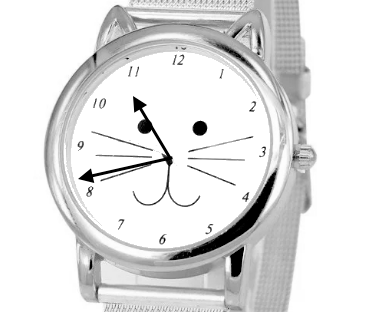
\includegraphics[width=5cm]{fig/relogioHoraPB}
\caption{Relógio marcando hora.}
\label{fig:relogio}
\end{center}
\end{figure}
\vspace{-0.5cm}
Quando realizamos uma medi\c c\~ao direta de uma grandeza, a partir da leitura de um instrumento anal\'ogico, que apresenta uma escala, o procedimento que se usa para fazer o registro do valor da grandeza \'e anotar todos os algarismos fornecidos pela escala do instrumento, eventualmente acrescentando mais um algarismo, que represente uma fra\c c\~ao da menor divis\~ao da escala do instrumento. No exemplo acima, do rel\'ogio, ao estimar 42 minutos, a pessoa imaginou uma escala de subdivis\~ao da menor divis\~ao do rel\'ogio em 5 partes, cada uma delas correspondendo a 1 minuto, e estimou que o ponteiro estava mais perto de duas subdivis\~oes. Quando o instrumento \'e digital, o m\'ultiplo da menor medida que ele pode fazer corresponde ao algarismo duvidoso do valor lido. Em um cron\^ometro digital com resolu\c c\~ao de 1 cent\'esimo de segundo, que mede um intervalo de tempo de 12,04 s, o 4 \'e o algarismo duvidoso da medida direta.

Um ponto que sempre gera dúvida é se os zeros são significativos ou não. Para responder, pense em alterar as unidades da medida. Se o número de zeros mudar ao fazer essa alteração, eles não são significativos, já que indicam apenas em que unidades estamos escrevendo a medida.  A medida ${x_1}=2,\!47$ cm tem três algarismos significativos, sendo o 7 duvidoso. Para escrever ${x_1}$ em metros, caminhamos a vírgula para a esquerda duas casas decimais e completamos com zeros. Nada foi feito em termos de alterar a quantidade de  informação em ${x_1}$, apenas trocamos as unidades, logo esses zeros de preenchimento não são significativos. Em resumo, as duas formas abaixo são equivalentes e têm três algarismos significativos:
\[
x_1=\underbrace{2,\!47}_{\mbox{\tiny sig}}\mbox{ cm} = 0,\!0\underbrace{247}_{\mbox{\tiny sig}}\mbox{ m}
\]
%
A mudança para uma unidade menor pode ser feita com ajuda de potências de dez, que não contam como algarismos significativos. Por exemplo, a medida ${x_2}$, com dois algarismos significativos pode ser escrita nas formas equivalentes
\[
{x_2}= 0,\!\underbrace{52}_{\mbox{\tiny sig}}\mbox{ kg} = 0,\underbrace{\!52}_{\mbox{\tiny sig}} \times 10^{3}\mbox{ g}  = \underbrace{5,\! 2}_{\mbox{\tiny sig}} \times 10^{2}\mbox{ g}
\]
%
Se escrevermos uma medida como ${x_3}=3,\!10$ s, ficará implícito que temos certeza dos três segundos e do um décimo de segundo. O zero na casa dos centésimos de segundo é duvidoso, sendo o último algarismo significativo da medida. Os zeros ao final do número são significativos. Observe mais um exemplo:
\[
\underbrace{100}_{\mbox{\tiny sig}}\mbox{ m}= 0,\underbrace{\!100}_{\mbox{\tiny sig}}\mbox{ km} = \underbrace{1,\!00}_{\mbox{\tiny sig}}\times 10^{8}\;\mu\mbox{m}
\]
%
Também aqui os dois algarismos zero à direita do 1 são significativos, independentemente da unidade que escolhamos para registrar o valor. Ao todo o comprimento registrado tem 3 algarismos significativos.

\section*{Incertezas e algarismos significativos}
%
%
Normalmente usamos um ou dois algarismos significativos para representar as incertezas, dependendo do grau de estimativa envolvido na sua determina\c c\~ao. Como vamos trabalhar com muitas estimativas na determina\c c\~ao das incertezas nas medidas diretas, usaremos a conven\c c\~ao de um significativo. Assim, o valor da medida deve ser escrito at\'e a casa decimal afetada pela incerteza, como nos exemplos abaixo.
%
\[
L = (2,\!25\pm 0,\!05)\mbox{ cm} \;\;\;\;\;\;\;\;  M = (351 \pm 2)\times 10^{-2}\mbox{ kg}
\]

No caso da incerteza de medidas indiretas, em geral \'e preciso arredondar o valor determinado a partir da propaga\c c\~ao das incertezas das medidas diretas, explicado no Capítulo~\ref{sec:medidasDir&Indir}.

Para arredondar um determinado valor,  vamos adotar os critérios da norma técnica da Associa\c c\~ao Brasileira de Normas T\'ecnicas ABNT-5891:
%
\begin{enumerate}
%
\item quando o algarismo a ser conservado for seguido de um algarismo inferior a 5, permanece inalterado o algarismo a ser conservado e retiram-se os posteriores (1,6357 arredondado à primeira casa decimal torna-se 1,6);
%
\item quando o algarismo a ser conservado for seguido de um algarismo superior a 5, ou igual a 5 seguido de no mínimo um algarismo diferente de zero, soma-se uma unidade ao algarismo a ser conservado e retiram-se os posteriores (1,6678 torna-se 1,7 e 1,6505 torna-se 1,7, arredondados à primeira casa decimal);
%
\item Se o algarismo à seguida do algarismo a ser conservado for igual a 5 e não houver mais nenhum algarismo à sua direita ou se todos os algarismos à direita forem zeros, retira-se todos os algarismos posteriores ao que será conservado e :
\begin{enumerate}
\item adiciona-se uma unidade ao algarismo conservado, se este for ímpar;
\item permanece inalterado o algarismo conservado, se este for par.
\end{enumerate}
%
\end{enumerate}
%
Observe os arredondamentos abaixo, feitos de modo a que a medida tenha 3 algarismos significativos e seguindo os critérios acima:
\begin{itemize}
%
\item $x = 4,678$ m $\rightarrow x = 4,\!68$ m 
\item $y = 4,674$ m $\rightarrow x = 4,\!67$ m 
\item $z = 4,675$ m $\rightarrow x = 4,\!68$ m  
\item $w = 4,665$ m $\rightarrow x = 4,\!66$ m 
%
\end{itemize}

Como exemplo, vamos calcular o peso $p$ da massa $m=(234,\!40\pm 0,02)$g sabendo que $g=(9,\!7879\pm 0,\!0001)$ m/s$^2$. 
Vamos trabalhar no SI, portanto escrevemos $m=(234,\!40\pm 0,\!02)\times 10^{-3}$ kg. Com isso,
%
\[
 p =  m \;   g = 2,\!29428376 \mbox{ N}
\]
%
Agora vamos calcular a incerteza. Como temos um produto,
\[
\left(\frac{\delta_p}{  p}\right)^2=\left(\frac{\delta_m}{  m}\right)^2+\left(\frac{\delta_g}{  g}\right)^2=\left(\frac{0,\!02}{234,\!00}\right)^2+\left(\frac{0,\!0001}{9,\!7879}\right)^2=7,\!409\times 10^{-10}
\]
Logo, 
\[
\delta_p=2,\!29428376 \mbox{ N}\times 2,\!72 \times 10^{-5}=6,\!23\times 10^{-5} \mbox{ N}
\]
Agora escrevemos a incerteza calculada com um significativo: 
\[
\delta_p = 6\times 10^{-5} \mbox{ N}
\]
Finalmente escrevemos $  p$ até a quinta casa decimal, usando o critério de arredondamento, e escrevemos o resultado final:
\[
2,\!2942\underline{8}376 \mbox{ N}\rightarrow p = (2,\!29428\pm 0,\!00006)\mbox{ N}
\]
%
Claro que também poderíamos usar a equação (\ref{eq:propag-geral}) para calcular a incerteza absoluta:
\[
\delta_p =  \sqrt{ (  m\delta_g)^2+(  g \delta_m)^2}.
\]
%
%\newpage
%


%

%\begin{comment}
%
%
%
\section*{Regra de bolso sobre algarismos significativos}
%
Muitas vezes o cálculo da incerteza propagada pode ser bem longo e fica difícil de saber se o resultado está certo ou não. Uma forma simples de saber se pelo menos a ordem de grandeza da incerteza propagada está correta é usar a seguinte regra:
%
\begin{itemize}
%
\item Numa operação matemática envolvendo medidas com diferentes números de algarismos significativos o resultado terá aproximadamente o mesmo número de algarismos significativos que a medida com menor número.
%
\end{itemize}
%
%

Vamos calcular o volume $V$ de um tubo de seção reta quadrada de lado $a=(2,\!0\pm0,\!1)$ cm e comprimento $L=(120,\!0\pm 0,\!1)$ cm.  
A medida $a$ tem 2 algarismos significativos e $L$, 4, sendo a mais precisa. Assim esperamos que $V$ tenha entre 2 e 4 algarismos significativos. Vamos fazer a propagação:
\[
V=a^2L\;\;\rightarrow\;\;   V =   a^2  L= 120,\!0\mbox{ cm}^3 
\]
%
\[
\left(\frac{\delta_V}{  V}\right)=\sqrt{\left(2\frac{\delta_a}{  a}\right)^2+\left(\frac{\delta_L}{  L}\right)^2}=0,\!1000034722
\]
Um erro muito comum é esquecer que 0,1000034722 é a incerteza  relativa e escrever este valor como se fosse a incerteza absoluta.

Calculando corretamente a incerteza absoluta, temos
\[
\delta_V=  V\left(\frac{\delta_V}{  V}\right)= (480,\!0\mbox{ cm}^3)( 0,\!1000034722) = 48,001666656 \approx 4,8001666656 \times 10  \mbox{ cm}^3
\]
Finalmente,
\[
V = (48\pm 5) \times 10 \mbox{ cm}^3\;
\]
O resultado final tem dois algarismos significativos, como a medida menos precisa usada no cálculo. Se for necessário melhorar a precisão da medida de $V$, vale a pena medir $a$ com mais precisão. Note que ao escrevermos o resultado final, utilizamos a mesma potência de 10 para $V$ e para sua incerteza $\delta_V$. Assim podemos saber qual deve ser o último algarismo a ser conservado no valor da medida e realizar o arredondamento, se necessário. Neste caso, o arredondamento foi feito na casa da unidade de $1\times 10 \mbox{ cm}^3$.
%

%\end{comment}
\section*{Exercícios}

%\vspace{-0.7cm}

Expresse corretamente os resultados para as seguintes medições com suas respectivas incertezas.
\begin{center}
\vspace{-1cm}
  \begin{tabular}{|c | c | c | c |>{ \centering\arraybackslash}m{8cm} |}  \hline
    & Medição	& Incerteza	& Unidades	& Resultado \\ \hline	 	
    1 & 67,002 & 0,023 & cm & \\ \hline
2 & 0,001 & 2,3 & erg & \\ \hline
3 & 45612,98 & 345 & cm/s & \\ \hline
4 & 14 & 29 & erg & \\ \hline
5 & 152,389 & 0,037 & cm/s$^2$ & \\ \hline
6 & 74,58 & 3,14 & g & \\ \hline
7 & 0,0012 & 0,0001 & m & \\ \hline
8 & 120034 & 2607 & m/s$^2$ & \\ \hline
9 & 45,98 & 2,1 & erg & \\ \hline
10 & 65555,467 & 56,001 & g & \\ \hline
11 & 23,456 & 1,2 & m & \\ \hline
12 & 0,173 & 0,056 & cm$^3$ & \\ \hline
13 & 45001,6 & 657,31 & J & \\ \hline
14 & 45,629 & 2,5914 & km/h & \\ \hline
15 & 104104 & 104 & m$^2$ & \\ \hline
16 & 0,0826 & 0,099 & cm/s & \\ \hline
17 & 3,69 & 1,582 & mm$^3$ & \\ \hline
18 & 19,78 & 5,46 & kg & \\ \hline
19 & 0,458 & 0,177 & cm & \\ \hline
20 & 135,589 & 0,0888 & g & \\ \hline
21 & 25,36 & 0,84 & cm & \\ \hline
22 & 74589,589 & 5698,26 & erg & \\ \hline
23 & 0,145 & 0,5 & cm/s & \\ \hline
24 & 14580,8 & 37,36 & erg & \\ \hline
25 & 125,369 & 0,041 & cm/s$^2$ & \\ \hline
26 & 74,58 & 3,14 & g & \\ \hline
27 & 0,025 & 0,0074 & m & \\ \hline
28 & 256 & 0,5 & m/s$^2$ & \\ \hline
29 & 7489 & 2,1 & m/s$^2$ & \\ \hline
30 & 4789,4 & 36,001 & g & \\ \hline   
  \end{tabular}
\end{center}


\begin{center}
  \begin{tabular}{|c | c | c | c |>{ \centering\arraybackslash}m{8cm} |}  \hline
    & Medição	& Incerteza	& Unidades	& Resultado \\ \hline	 
18 & 19,78 & 5,46 & kg & \\ \hline
19 & 0,458 & 0,177 & cm & \\ \hline
20 & 135,589 & 0,0888 & g & \\ \hline
21 & 25,36 & 0,84 & cm & \\ \hline
22 & 74589,589 & 5698,26 & erg & \\ \hline
23 & 0,145 & 0,5 & cm/s & \\ \hline
24 & 14580,8 & 37,36 & erg & \\ \hline
25 & 125,369 & 0,041 & cm/s$^2$ & \\ \hline
26 & 74,58 & 3,14 & g & \\ \hline
27 & 0,025 & 0,0074 & m & \\ \hline
28 & 256 & 0,5 & m/s$^2$ & \\ \hline
29 & 7489 & 2,1 & m/s$^2$ & \\ \hline
30 & 4789,4 & 36,001 & g & \\ \hline
  \end{tabular}
\end{center}
